% this shell was created by
% Guillaume R. Frechette
% it is a modification of the Standard LaTex Article (Harvard) shell


\documentclass[11pt]{article}
%%%%%%%%%%%%%%%%%%%%%%%%%%%%%%%%%%%%%%%%%%%%%%%%%%%%%%%%%%%%%%%%%%%%%%%%%%%%%%%%%%%%%%%%%%%%%%%%%%%%%%%%%%%%%%%%%%%%%%%%%%%%%%%%%%%%%%%%%%%%%%%%%%%%%%%%%%%%%%%%%%%%%%%%%%%%%%%%%%%%%%%%%%%%%%%%%%%%%%%%%%%%%%%%%%%%%%%%%%%%%%%%%%%%%%%%%%%%%%%%%%%%%%%%%%%%
\usepackage{amsfonts}
\usepackage{graphicx}
\usepackage{amsmath}
\usepackage{float}
\usepackage{natbib}
\usepackage{endnotes}
\usepackage{doublespace}
\usepackage{booktabs} % For formal tables
\usepackage[ruled]{algorithm2e}
\renewcommand{\algorithmcfname}{ALGORITHM}
\SetAlFnt{\small}
\SetAlCapFnt{\small}
\SetAlCapNameFnt{\small}
\SetAlCapHSkip{0pt}
\IncMargin{-\parindent}
\SetKw{Initialize}{initialize}
\SetKw{Trace}{traceback}
\SetKw{Set}{set}
\SetKw{Return}{return}
\setcounter{MaxMatrixCols}{10}
%TCIDATA{OutputFilter=LATEX.DLL}
%TCIDATA{<META NAME="SaveForMode" CONTENT="1">}
%TCIDATA{Created=Mon Jun 10 12:02:11 2002}
%TCIDATA{LastRevised=Mon Jun 10 12:48:41 2002}
%TCIDATA{<META NAME="GraphicsSave" CONTENT="32">}
%TCIDATA{<META NAME="DocumentShell" CONTENT="Journal Articles\apsa">}
%TCIDATA{Language=American English}
%TCIDATA{CSTFile=LaTeX article (bright).cst}

\setlength{\textwidth}{6.5in} 
\setlength{\textheight}{8in} 
\setlength{\oddsidemargin}{0.5in}
\setlength{\topmargin}{0in}
\setcounter{secnumdepth}{-1}
\makeatletter
\renewcommand{\section}{\@startsection 
{section}{1}{\z@}{3.5ex plus -1ex minus -.2ex}{2.3ex plus .2ex}{\centering\normalsize\bf}}
\renewcommand{\subsection}{\@startsection 
{subsection}{2}{\z@}{3.25ex plus -1ex minus -.2ex}{1.5ex plus .2ex}{\normalsize\bf}}
\renewcommand{\subsubsection}{\@startsection 
{subsubsection}{3}{\z@}{3.25ex plus -1ex minus -.2ex}{1.5ex plus .2ex}{\raggedright\normalsize\underline}}
\def\enoteformat{\raggedright
\parindent=1.8em
     \leavevmode\llap{\hbox{$^{\@theenmark}$}}}
\makeatother
\renewcommand{\footnote}{\endnote} 
\newtheorem{theorem}{Theorem}
\newtheorem{acknowledgement}[theorem]{Acknowledgement}
\newtheorem{axiom}[theorem]{Axiom}
\newtheorem{case}[theorem]{Case}
\newtheorem{claim}[theorem]{Claim}
\newtheorem{conclusion}[theorem]{Conclusion}
\newtheorem{condition}[theorem]{Condition}
\newtheorem{conjecture}[theorem]{Conjecture}
\newtheorem{corollary}[theorem]{Corollary}
\newtheorem{criterion}[theorem]{Criterion}
\newtheorem{definition}[theorem]{Definition}
\newtheorem{example}[theorem]{Example}
\newtheorem{exercise}[theorem]{Exercise}
\newtheorem{lemma}[theorem]{Lemma}
\newtheorem{notation}[theorem]{Notation}
\newtheorem{problem}[theorem]{Problem}
\newtheorem{proposition}[theorem]{Proposition}
\newtheorem{remark}[theorem]{Remark}
\newtheorem{solution}[theorem]{Solution}
\newtheorem{summary}[theorem]{Summary}
\newenvironment{proof}[1][Proof]{\textbf{#1.} }{\ \rule{0.5em}{0.5em}}
\setlength{\parindent}{4em}

\begin{document}

\title{Text reuse and Paraphrase Detection with Semantical Smith-Waterman Local Alignment}
\author{Alexander Furnas}

\date{}
\maketitle

\pagebreak  
%TCIMACRO{\TeXButton{beginflushleft}{\begin{flushleft}} }%
%BeginExpansion
\begin{flushleft}
%EndExpansion
%TCIMACRO{\TeXButton{worddouble}{\setstretch{1.805}\small\normalsize} }%
%BeginExpansion
\setstretch{1.805}\small\normalsize
%EndExpansion


%TCIMACRO{\TeXButton{beginabstract}{\begin{abstract}}}%
%BeginExpansion
\begin{abstract}%
%EndExpansion
Coordination among political elites is an issue of substantive interest across political science. This paper details a new method for detecting text reuse and paraphrasing in political texts, a critical measurement task in leveraging new text data to observe patterns of coordination. The method proposed is an extension of the Smith-Waterman local alignment algorithm with semantically aware mismatch penalties. This modification enables detection of instances of text reuse in which words are changed to semantically similar alternatives to fit new contexts or disguise the source of the text. This method is applied to a corpus of tweets sent by Members of Congress and their electoral challengers during the 2016 election cycle.%TCIMACRO{\TeXButton{endabstract}{\end{abstract}}}%
%BeginExpansion
\end{abstract}%
%EndExpansion
\pagebreak
\setlength{\parskip}{1em}
\setlength{\parindent}{4em}
\section{Motivation}

 Studies of congressional behavior have long focused on the motivations of Members of Congress. \cite{fenno1978home} famously argues that members are motivated by three primary goals: re-election, power within the institution, and good public policy. To achieve these goals they may collaborate or coordinate with other members. There has been substantial theoretical work exploring members voting decisions \citep{kingdon1977models}, allocation of attention to issues \citep{hall1998participation, hall2006lobbying}, and how they communicate with their constituents \citep{miller1963constituency, mayhew1974congress}.  Following \cite{mayhew1974congress}, scholars have focused largely on how re-election motivation shapes legislators representation behavior. Recent work in using text analysis has looked at how members represent their work in Washington to their constituents \citep{grimmer2010bayesian}, and tested longstanding theories of distributive politics and credit claiming \citep{grimmer2012words}.

Members share the primary goals of re-election, institutional prestige and public policy outcomes with each other in varying degrees. While the between member coherence may vary just as their ideologies, constituencies and aspirations do, the existence of shared goals creates the opportunity for productive collaboration. Indeed, the \cite{cox2005setting} conceive of parties in the House as collaborative undertaking to protect a re-electable party brand by controlling the agenda. The bargaining within legislatures that enables logrolling and undergirds distributive theories of legislative organization is necessarily a collaborative and coordinated process \citep{baron1989bargaining, shepsle1987institutional, berry2015cardinals}.

Indeed, we may think of different types of collaboration and coordination that support members differing goals, ambitions and styles. A substantial body of work has explored how members collaborate by cosponsoring legislation \citep{zhang2008community,fowler2006connecting, koger2003position}. \cite{koger2003position} argues that cosponsorship serves as a form of position taking and as a signal to agenda-setters. \cite{campbell1982cosponsoring} finds that legislators cosponsor bills for ideological, partisan, and electoral reasons, suggesting that they see this form of cooperation as meaningful in achieving their goals.\cite{fowler2006connecting} shows that centrality in the cosponsorship network is predictive of legislative effectiveness. Cosponsorship can send messages of bipartisanship to obstructionist minorities \citep{wilson1997cosponsorship}. At the state level \cite{bratton2011networks} find that ideology and homophily predict cosponsorship between legislators. Legislators use cosponsorship to signal to constituents, help pass policy they support and increase their standing within the institution. This form of coordination and collaboration between Members of Congress is an essential part of legislative behavior.

Recent work by \cite{craig2015room} has explored between Member collaboration in Dear Colleague letters, a semi-formalized system of member-to-member communication used for information sharing, cosponsorship recruitment, issue advocacy or administrative or operational communication. \cite{craig2015room} finds a significant degree of bipartisan collaboration in the Dear Colleague network and \cite{craig2015cue} finds that letters can have an impact on the legislative success of a bill. In this too, Members' are coordinating and collaborating with each other in pursuit of their goals.

In recent years, scholars in political science have begun using natural language processing techniques to analyze vast troves of politically relevant text \citep{grimmer2013text}. This work has applied techniques ranging from topic modeling \citep{roberts2014structural} to scaling to recover latent traits \citep{lowe2013validating}. 

\cite{lin2014burst} use distinctive n-grams in member communications over time to detect ``semantic bursts" of coordinated among Senators, and find that these coordinated communication networks reflect underlying institutional and partisan factors. \cite{lin2015uncovering} explore how differing the reuse and diffusion of different length n-grams reflect different behavioral processes within the chamber.

A recent body of work has begun explicitly to detect text reuse in political texts, particularly for modeling diffusion or policy \citep{smith2013infectious,smith2014detecting, wilkerson2015tracing, Furnas2017ideal, Fridolin2017text}. The detection of text-reuse offers an exciting new means for exploring the patterns of collaboration and coordination among political actors. 

\cite{wilkerson2015tracing} detect reuse of legislative language from previously introduced bills in the Affordable Care Act. Their suggested re-framing of legislative behavior from bill to policy-idea as a meaningful unit of analysis suggests a greater degree of ideological diversity in ACA, and offers exciting new avenues for the study of legislative effectiveness. More recently, \cite{burgess2016legislative,Fridolin2017text} look at how legislative text is shared and reused between states. \cite{Furnas2017ideal} use the same instances of text reuse to construct new bridges for cross state ideal point estimation.

\cite{wilkerson2015tracing, burgess2016legislative,Fridolin2017text} and \cite{Furnas2017ideal} all use the same algorithm for identifying text reuse: the Smith-Waterman local alignment algorithm. The Smith-Waterman algorithm was originally developed in biostatistics to find the optimal local alignments of sequences of nucleic acids \cite{smith1981identification}. Work by\cite{smith2013infectious,smith2014detecting} has adapted the Smith-Waterman local alignment algorithm (SW, hereafter) for text purposes.


SW is an effective algorithm for finding examples of exact text reuse, or reuse of exact text with additional text insertions. A global text alignment algorithm, like the Needleman-Wunsch, would do a poor job of detecting text from string $A$ reused in string $B$, if $B$ were identical to $A$ but with a new appositional phrase inserted in the middle\cite{needleman1970general}. 

SW is a dynamic programming algorithm that computes all of the possible alignments of two sequences, tabulating scores according to a bonus for aligned items, a penalty for mismatching items and a penalty for the insertion of gaps. Backpointers to previous parts of the alignment are stored in a table. The maximum possible score is found, and then backpointers are used to determine what path of the possible alignments yielded that optimal alignment. In this way it is similar to an edit distance calculation. All misalignments, that is cases where words in the two sequences do not match, are treated the same. \cite{Fridolin2017text} provides an extensive explanation of the algorithm for political science audiences.

To date, SW has been by political scientists used largely to detect the reuse of legislative text. In a legislative context, where changing a single ``shall" to a ``may" can significantly alter the meaning of a provision, exact matches may be the appropriate form of text reuse to detect. However, in other forms of political text or speech we may be interested in a more flexible form of text reuse. SW is less effective for detecting instances of reuse in which moderate paraphrasing or adaptation has been done. This is especially relevant in the context of political speech, as two actors offering essentially the same message may need to adapt it to fit their circumstances. 

As text reuse detection becomes an increasingly common tool to detect patterns of coordination and collaboration among political actors --- beyond legislative language --- I argue that a more flexible tool is necessary. 


I propose a modification of the standard SW algorithm in to better detect this adaptive reuse. This modified version is called the Semantic Smith-Waterman (SSW. hereafter). Rather than treating all mismatches the same, the method proposed here scores each mismatch according to word similarity in a semantic space and weights these mismatches accordingly. The more similar the two words are the less the mismatch is penalized. While I explore only a simple semantic distance weighting here, this simple modification enables a variety of more complex and semantically meaningful penalization schemes. 


\section{Method}


Consider a hypothetical legislator expressing  one of the following sentiments:

\textbf{A:} \emph{"My esteemed colleague is resident of the state of Michigan, and clearly proud of it."}
 
\textbf{B:} \emph{"My esteemed colleague is resident of the state of denial, and clearly proud of it."}
 
In statement A, the legislator is making a straightforward statement about the state of residence of their colleague. In statement B, the legislator is making an ironic statement about their colleague's inability to confront facts. While the text in these two instances is almost exactly the same, their meanings are notably different. 

Now consider a second hypothetical legislator, making the following statement: 

\textbf{C:} \emph{"My esteemed colleague is resident of the state of Ohio, and clearly proud of it."}

Is statement C more similar to A or B? The standard SW algorithm would say that C is equally as similar to A as it is to B. C aligns with A and B perfectly except for one mismatch (``Michigan" --- ``Ohio" and ``denial" --- ``Ohio") which are penalized equally according to a constant.

The SSW scores these differently. The mismatch penalty applied depends on the relationships between the words in a semantic space. In the application of SSW presented here, words are compared in a google's pre-trained 300 dimension \texttt{word2vec} word embeddings. These vector space word representations are pre-trained according to the method described by \cite{mikolov2013efficient} using the google news corpus. However, a future more general application will present the possibility of using a variety of vector spaces. For example, it may be useful to construct a custom latent semantic space out of the corpus of documents being analyzed using Latent Semantic Analysis \citep{furnas1988information, deerwester1990indexing}. The algorithm presented here can be simply adapted for any custom vector space representation of words.

Algorithm \ref{alg:one} provides a detailed explication of the the SSW algorithm. The algorithm functions nearly identically to the standard SW, except that mismatches are scored according to a similarity function rather than penalized with a constant. The similarity score $s(a,b)$ for two words $a$ and $b$ is derived according to the scoring function described in Algorithm \ref{alg:semsim}.

The SSW consists of the same four steps as SW:

\begin{enumerate}
\item Choice of scoring parameters.
\item The scoring and traceback matrices are initialized,
\item The scoring matrix is filled, and backpointers stored in the traceback matrix
\item Traceback starting from the highest scoring cell in the scoring matrix.

\end{enumerate}


\begin{algorithm}[t]
\SetAlgoNoLine
\KwIn{Two sequences of words, $A$ and $B$, such that $A=a_{1}a_{2}... a_{n}$ and $B=b_{1}b_{2}... b_{m}$ where $n$ and $m$ are the lengths of $A$ and $B$ respectively.}
\KwOut{Optimal semantically aware local alignment of A and B with gaps, alignment score}
\vspace{10pt}

\Initialize{Scoring matrix $\mathbf{H}$}{ with dimensions $(n+1) \times (m+1)$, \\ \hspace{33pt}$ H_{k0}=H_{0l}=0\quad for\quad 0\leq k\leq n\quad and\quad 0\leq l\leq m$;} 

\Initialize{Traceback matrix $\mathbf{T}$}{ with dimensions $(n) \times (m)$;}
\vspace{10pt}

 \For{each node $i$ in $j$ in $1:n+1, 1:m+1$}{
 
 \hspace{1em}${\displaystyle H_{ij}=\max {\begin{cases}H_{i-1,j-1}+s(a_{i},b_{j}),\\H_{i-1,j}-W,\\H_{i,j-1}-W,\\0\end{cases}}}$
 
\vspace{10pt} 
\textbf{where:}

 \hspace{1em}$H_{i-1,j-1}+s(a_{i},b_{j})$ is the semantically weighted score of aligning $a_{i}$ and $b_{j}$,

 \hspace{1em}$H_{i-1,j}-W_{1}$ is the score if $a_{i}$ is at the end of a gap,

 \hspace{1em}$H_{i,j-1}-W_{1}$ is the score if $b_{j}$ is at the end of a gap,


\vspace{10pt}

 \hspace{1em} ${\displaystyle T_{ij}={\begin{cases}    (i-1,j-1), & \text{if } H_{ij} = H_{i-1,j-1}+s(a_{i},b_{j}) \\
    (i-1,j), & \text{if } H_{ij} = H_{i-k,j}-W \\
    (i,j-1), & \text{if } H_{ij} = H_{i,j-l}-W
    \end{cases}}}$
}
\vspace{10pt}

\Trace{Starting at $H_{ij}$ = $max(\mathbf{H})$}{\\
 \hspace{1.55em}alignment = [ ]

\While{$H_{ij} > 0$}{
append $T_{ij}$ to alignment

\Set{$i$,$j$}{ to $T_{ij}$}}
 
}

\Return{score = $max(\mathbf{H})$, alignment = alignment}

\caption{Semantic Smith Waterman \protect\footnotemark}
\label{alg:one}
\end{algorithm}

\footnotetext{Notation and explication for the Semantic Smith-Waterman used here is adapted from the Wikipedia article for the standard Smith-Waterman.} 


\subsection{Semantic mismatch scoring}
At this point it some additional explanation of the semantic mismatch scoring used here is warranted at is the principal difference between SW and SSW. Standard SW generally imposes a constant penalty for a mismatch, and then either a linear penalty for gap scoring or an affine gap penalty (where there is a greater penalty for creating than extending a gap). Both \cite{wilkerson2015tracing} and \cite{Fridolin2017text} use affine gap scoring versions of SW. For the sake of simplicity the proof-of-concept implementation described here uses linear gap penalty, but there is no reason that SSW could not be extended to include affine gap scoring. A forthcoming python package that implements SSW will include an affine gap option.

This implementation makes a few other simplifying assumptions that could be parameterized in a future implementation of SSW. These are as follows:

\begin{itemize}
\item Cosine similarity of word vectors in the\texttt{word2vec} semantic space is used as the similarity measure. 
\item Cosine similarity scores below .5 are considered a mismatch and standard constant mismatch penalty is applied.
\item The constant mismatch penalty is set to be the same as the constant gap penalty $W$.
\item Perfect matches are set given a positive score twice the magnitude of the gap/mismatch penalty.\footnote{This matches the most common or default ratio between gap and match penalties uses in most applications of the standard SW.}
\end{itemize}
  
Algorithm \ref{alg:semsim} shows this implementation. Here, $\mathbf{V}$ is a vector space from the \texttt{word2vec} word embeddings. 

\begin{algorithm}[t]
\SetAlgoNoLine
\KwIn{Two words, $a$ and $b$, semantic vector space $\mathbf{V}$, and baseline weight $W$.}
\KwOut{An alignment score, $s(a,b)$ to be used in the Semantic Smith-Waterman alignment}
\If{$a=b$}{score $= 2W$}
\ElseIf{$a$ is a stop word or $b$ is a stop word}{score $= -W$}
\Else{$s= \cos(\mathbf{V}[a], \mathbf{V}[b]) -.5$

score$ =  2W s$ }
\caption{Semantically Weighted Alignment Score}
\label{alg:semsim}
\end{algorithm}

\subsection{Initialization}
The scoring matrix is initialized to with the words from string $A$ along the rows and from string $B$ along the columns, but with a first row and column set to 0. The result is a matrix with dimensions $(n+1)\times (m+1)$. Here, $n$ is the number of words in $A$ and $m$ is the number of words in $B$. The traceback matrix is initialized to be size $n \times m$. 

\subsection{Scoring}
As cells in the scoring matrix are filled,as shown in Figure \ref{fig:score}, a pointer is stored in the traceback matrix indicating which of the neighboring cells provided the max value for $H_{i,j}$.

\begin{figure}
\centering
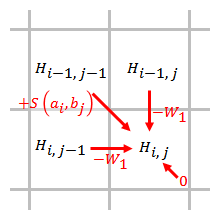
\includegraphics[width=.4\textwidth]{Smith-Waterman-Algorithm-Scoring-1.png}
\caption{Scoring and Traceback. Source: Wikimedia Commons}
\label{fig:score}
\end{figure}

\footnotetext{Notation and explication for the Semantic Smith-Waterman used here is adapted from the Wikipedia article for the standard Smith-Waterman.} 

\subsection{Traceback}
The cell in the traceback matrix that corresponds to the cell in the scoring matrix which provides the maximum value is used as the starting position for traceback. Starting from this cell, the backpointers are used to determine the optimal local alignment of the two strings. Backtracing ends when the corresponding cell in the scoring matrix reaches 0.

\section{Empirical application}
To explore the utility of this new approach to text reuse detection, I applied both SW and SSW to a corpus of tweets of Members of Congress and congressional candidates during the 2016 election cycle.\footnote{These tweets were kindly shared with me by Joseph DiGrazia, and when he publishes something with this corpus, any work that I produce validating this measure using this corpus will cite him.}

This corpus contains $893168$ non-retweet tweets from $714$ different accounts. Of these I took the first $100000$ tweets and looked for optimal local alignments in the rest of the $893168$ tweet corpus with both SW and SSW. These algorithms are computationally expensive, as they are $O(nm)$. Checking for each optimal alignment would require this be done $100000 \times 893168 \approx 8.93 \times 10^{10}$ times. 

To shrink the search space, I compared all documents to each other in a simple vector space constructed using \texttt{nltk} and \texttt{gensim} in python \citep{bird2006nltk, rehurek2010lrec}. Because I wanted to find results with as similar exact words as possible to each other, I did no transformations on this vector space, and did not remove stop words. Each tweet was then compared to the 100 closest tweets in this vector space using both SW and SSW. The scaling parameter used as the baseline gap penalty $W$ was set to 10 for these trials.

Below I present the distributions of these similarity scores. Note, of course, that the sample of similarity scores calculated is a non-random sample of similarities between these tweets because of how the search space was constrained. As Figure \ref{fig:scoredist} shows, these scores are highly similar, of course, but the interesting results come in the instances where SSW is substantially different from SW. 


\begin{figure}
\centering
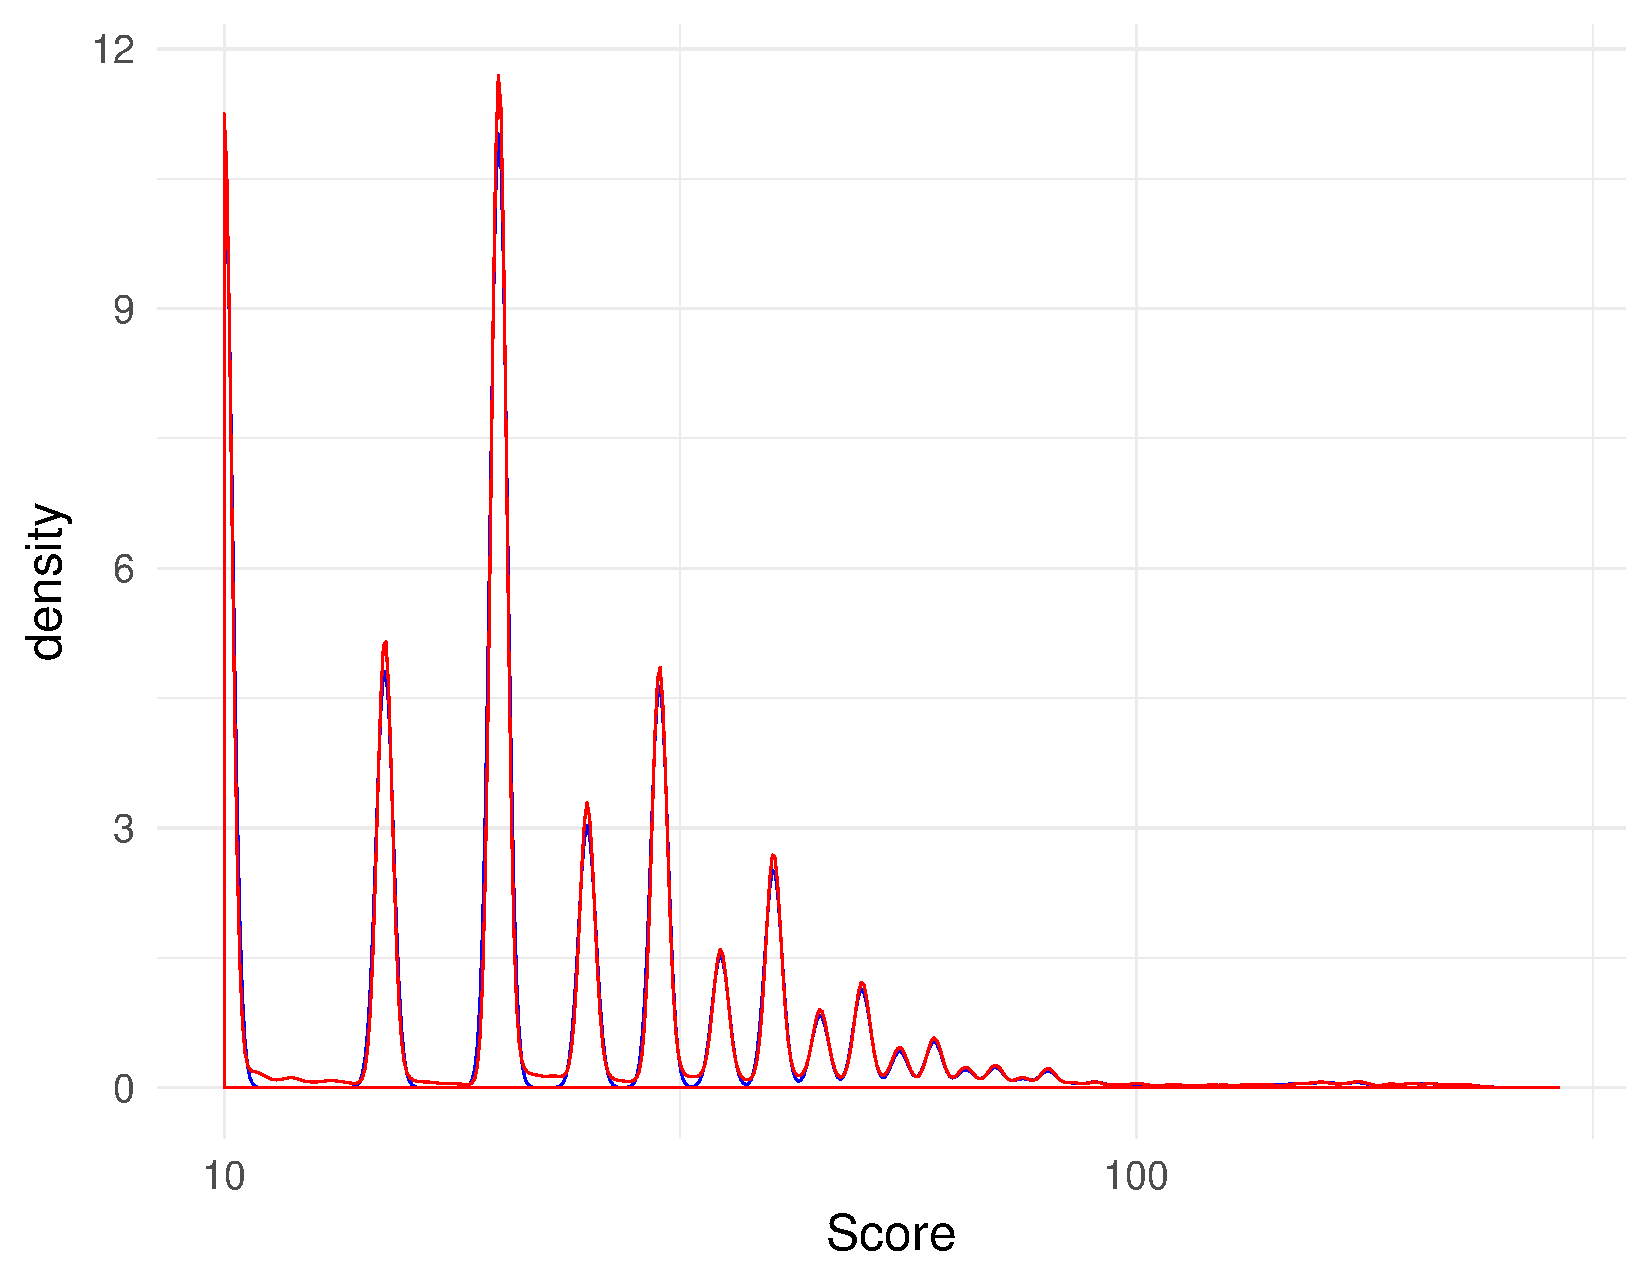
\includegraphics[width=.6\textwidth]{Score_densities.pdf}
\caption{Smith-Waterman and Semantic Smith-Waterman Score densities}
\label{fig:scoredist}
\end{figure}


Filtering the set of tweets to dyads with similarity scores above 90  --- the equivalent of a 9 word reuse sequence --- leaves a set of 144,031 tweets. We can observe substantial variation between the SSW and SW scores here. The two distributions converge above about 190, perfect matches at the tweet length limit. 

\begin{figure}
\centering
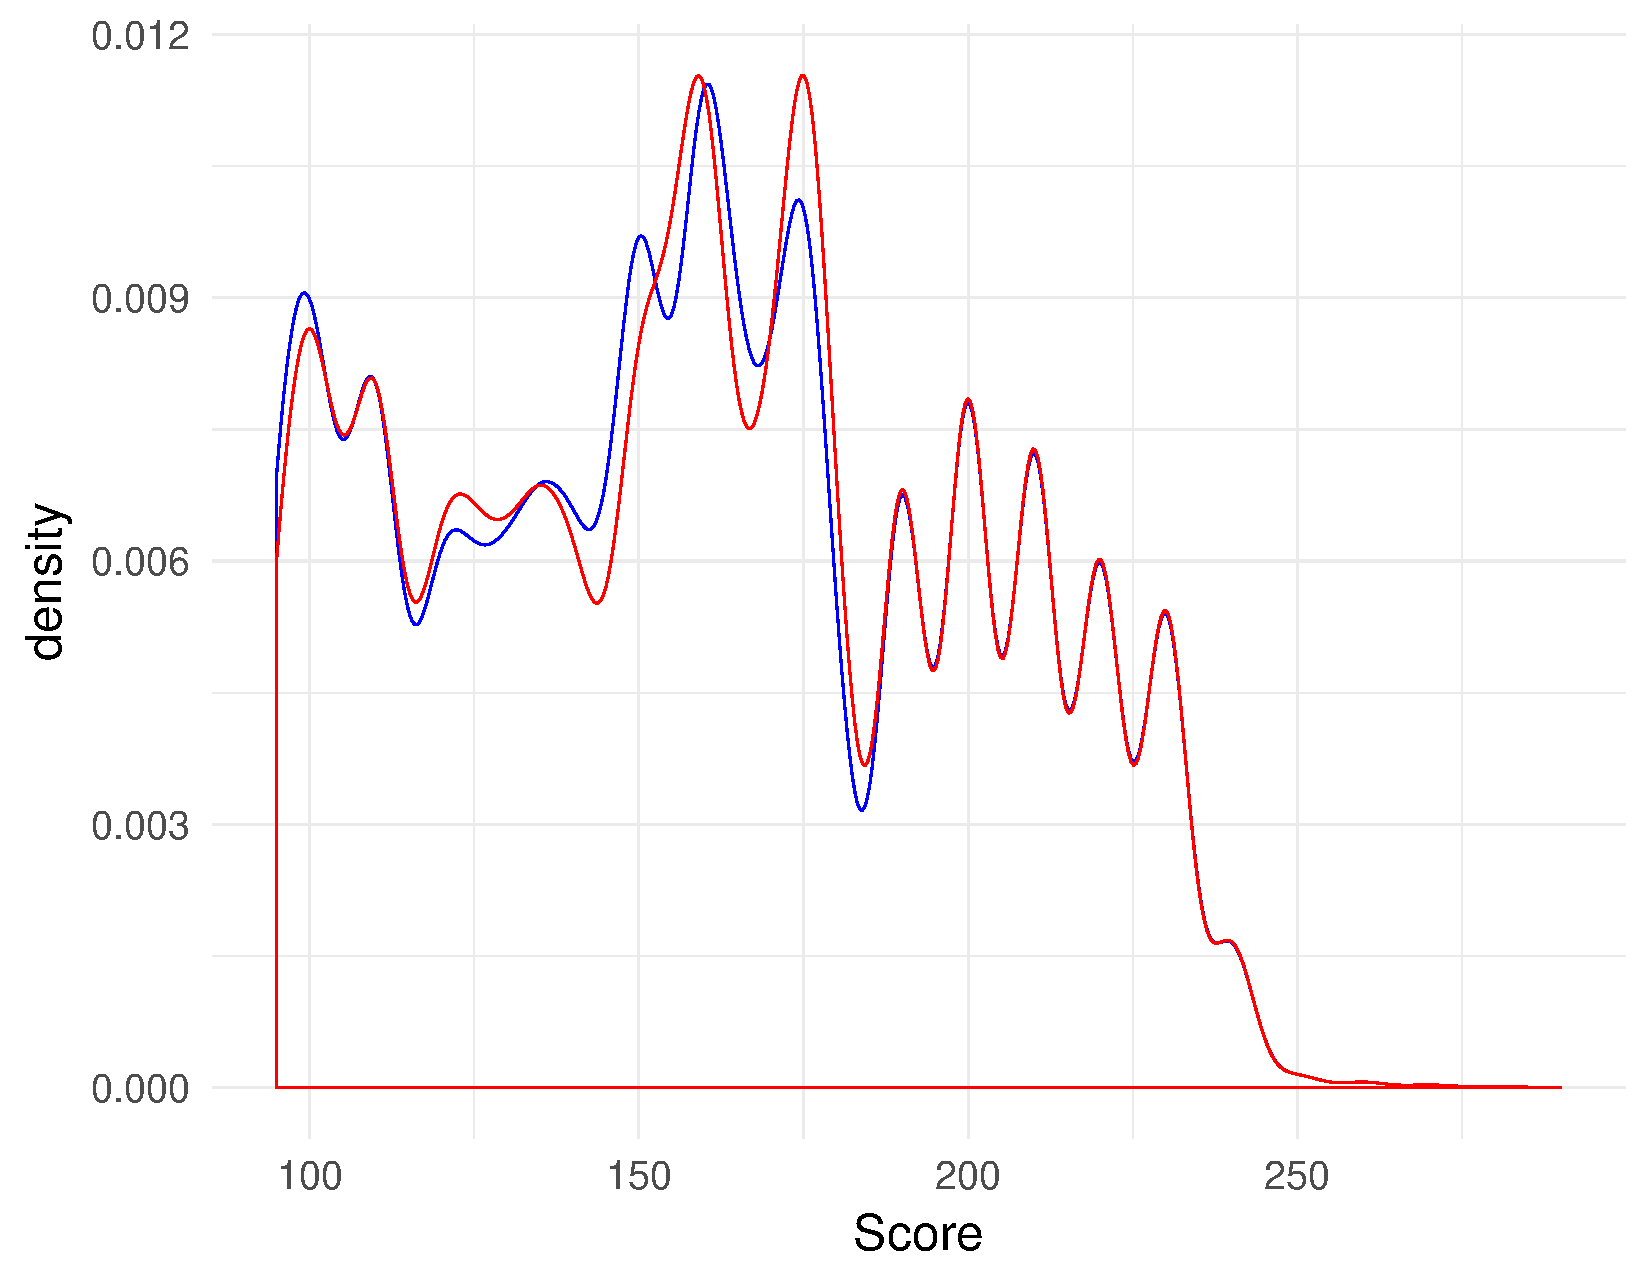
\includegraphics[width=.6\textwidth]{Above_90_Scores.pdf}
\caption{Smith-Waterman and Semantic Smith-Waterman Score densities above 90}
\label{fig:scoredist}
\end{figure}


SSW yields strictly higher scores than SW, as the semantic similarity score defaults to the standard mismatch penalty if the semantic similarity score is negative. The distribution of these differences is shown in Figure \ref{fig:scorediff} for all cases where that difference is non-zero.

\begin{figure}
\centering
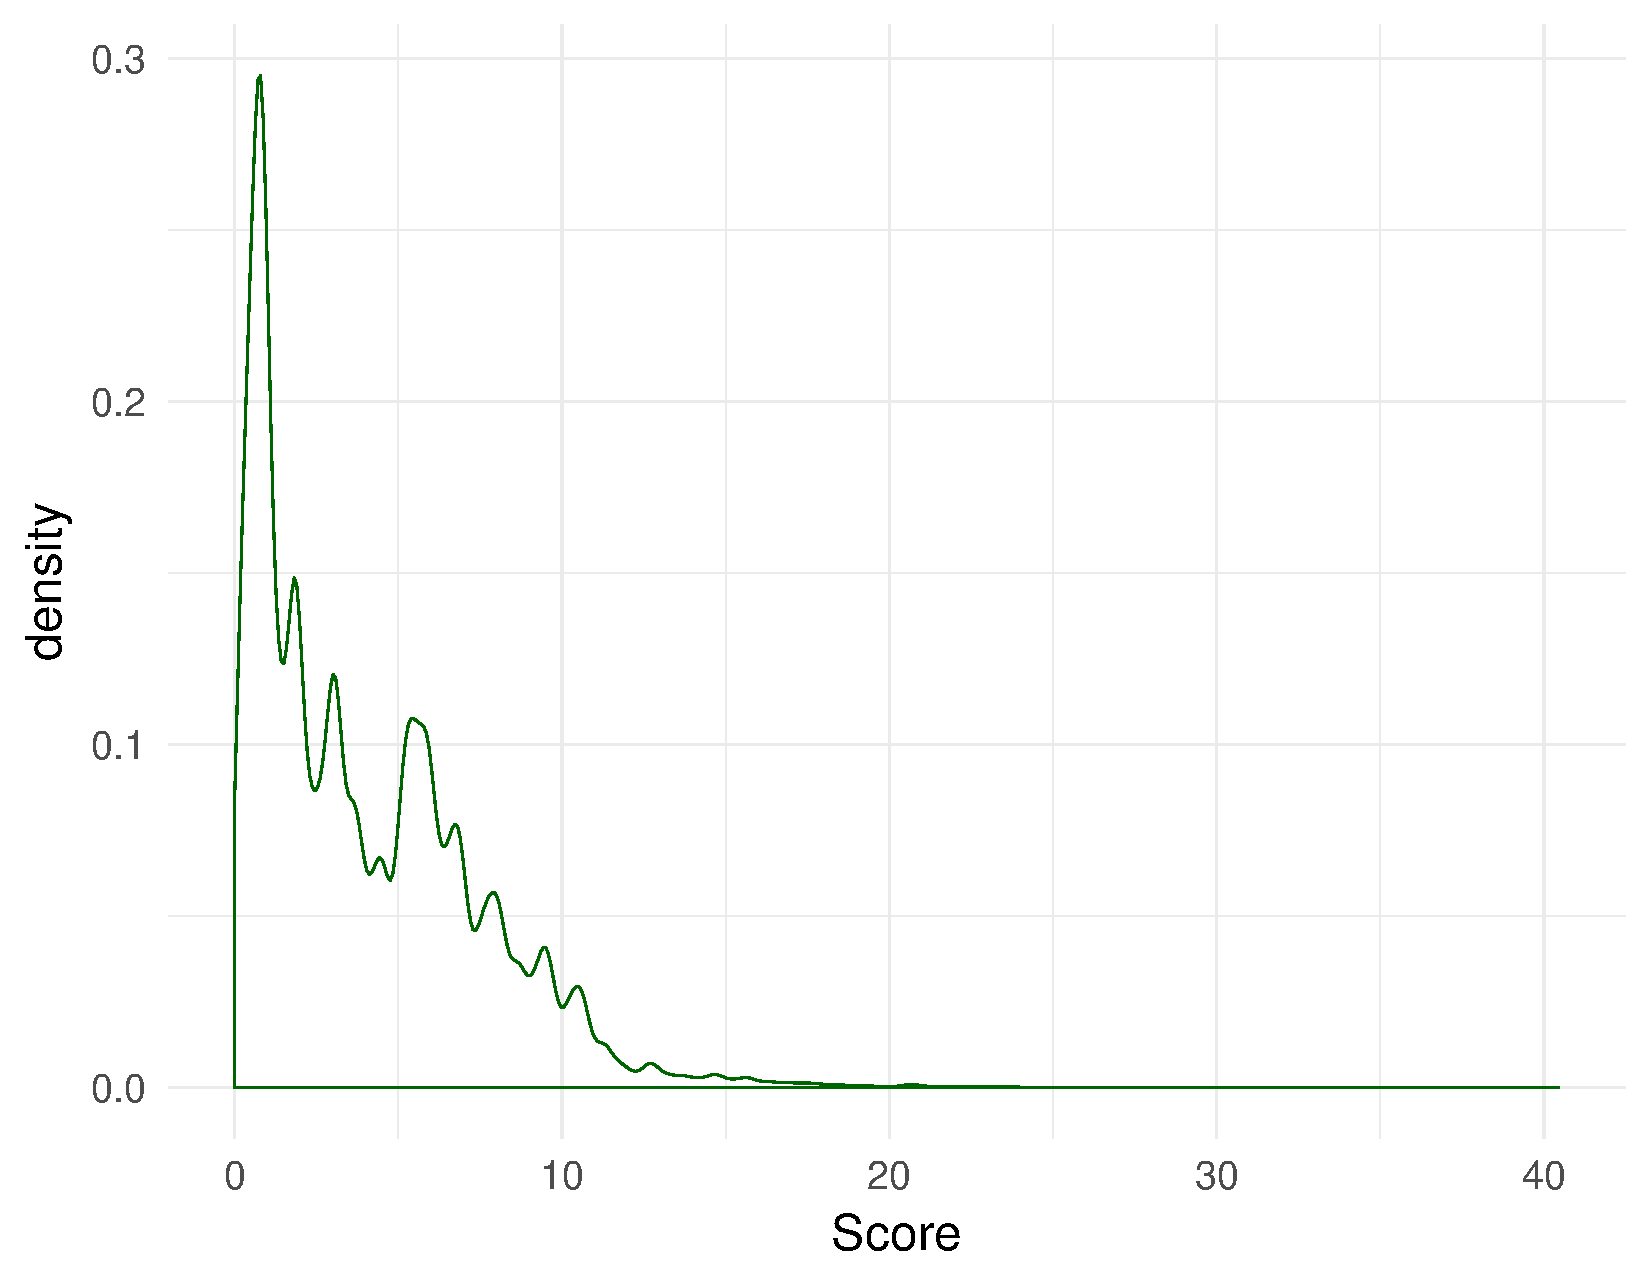
\includegraphics[width=.6\textwidth]{Score_Diff.pdf}
\caption{Density of difference between Smith-Waterman and Semantic Smith-Waterman Score densities}
\label{fig:scorediff}
\end{figure}

Tables \ref{tbl:diff} and \ref{tbl:diff2} provide a sample of tweet interesting tweet comparisons using SW and SSW. Those provided below are the top 50 tweets with SW scores above 90, sorted by the magnitude of the difference in their SW and SSW scores. They provide a useful illustration of the kinds of similarity that SSW can help detect that SW does not. For example, the tweet ``Thank you to all brave men and women serving our nation and keeping us safe. \#ArmedForcesDay https://t.co/xVswnTWMR0" and ``Thank you to all of the brave men and women who serve our country and keep us safe. \#ArmedForcesDay" express the same semantic content, but have been phrased slightly differently. SSW yields a score that is the equivalent of nearly 3 additional overlapping words. 

Similarly, the tweet ``My thoughts and prayers are with the victims, their families and all those affected by the attack in Orlando." contains the same meaningful semantic content as ``My thoughts and prayers are with the victims, the injured, their families and all others impacted by today's senseless attacks in \#Boston." but is adapted to fit a different context following a different attack. The virtue of SSW is in detecting the use of similar phrasing adapted to new contexts in this manner.  

A closer examination of the tweet pair presented in tables \ref{tbl:diff} and \ref{tbl:diff2} reveals some interesting themes. We see members responding with similar content to crises, breaking news, political and calendar events. In many cases, semantic meaning is identical but minor phrasing variations exist between members, often using different patterns of hash-tagging. SSW presents the possibility of detecting coordinated messaging despite the kinds of changes social media interns may introduce to fit with members goals and homestyles.

As a further demonstration of the utility of this tool, I have conducted a simple descriptive network analysis of similar tweet dyads. Figure \ref{fig:tweetnet} shows the network of similar tweets between the Members of Congress and their challengers during the 2016 election cycle. The set of dyads which were compared using SSW was subset to include only dyads which scored above 105 (the minimal score included in tables \ref{tbl:diff} and \ref{tbl:diff2}). These dyads were considered to be an instance of shared messaging. 

I then summed the number of tweet dyads above this threshold between each pair in the sample to derive a weighted edge between them. It is worth noting that while tweets from incumbent members sent 74.32 percent of the 893,168 tweets in the sample, they sent 97.05 percent of the tweets in the 13,489 dyads that surpass the 105 similarity threshold with other tweets.\footnote{It should be noted that some tweets are counted multiple times here, if they show up in multiple dyads.} Members of Congress appear to tweet much more similarly to each other than they do to their challengers. Figure \ref{fig:tweetnet} shows the network of these shared tweets, with actors colored by their party. Descriptively we can see that actors tend to share tweets with their co-partisans more frequently than out-partisans. It is interesting to note, however, that the degree of separation between these two communities is less than we tend to observe in other political networks like co-sponsorship, voting in Congress.



\begin{figure}
\centering
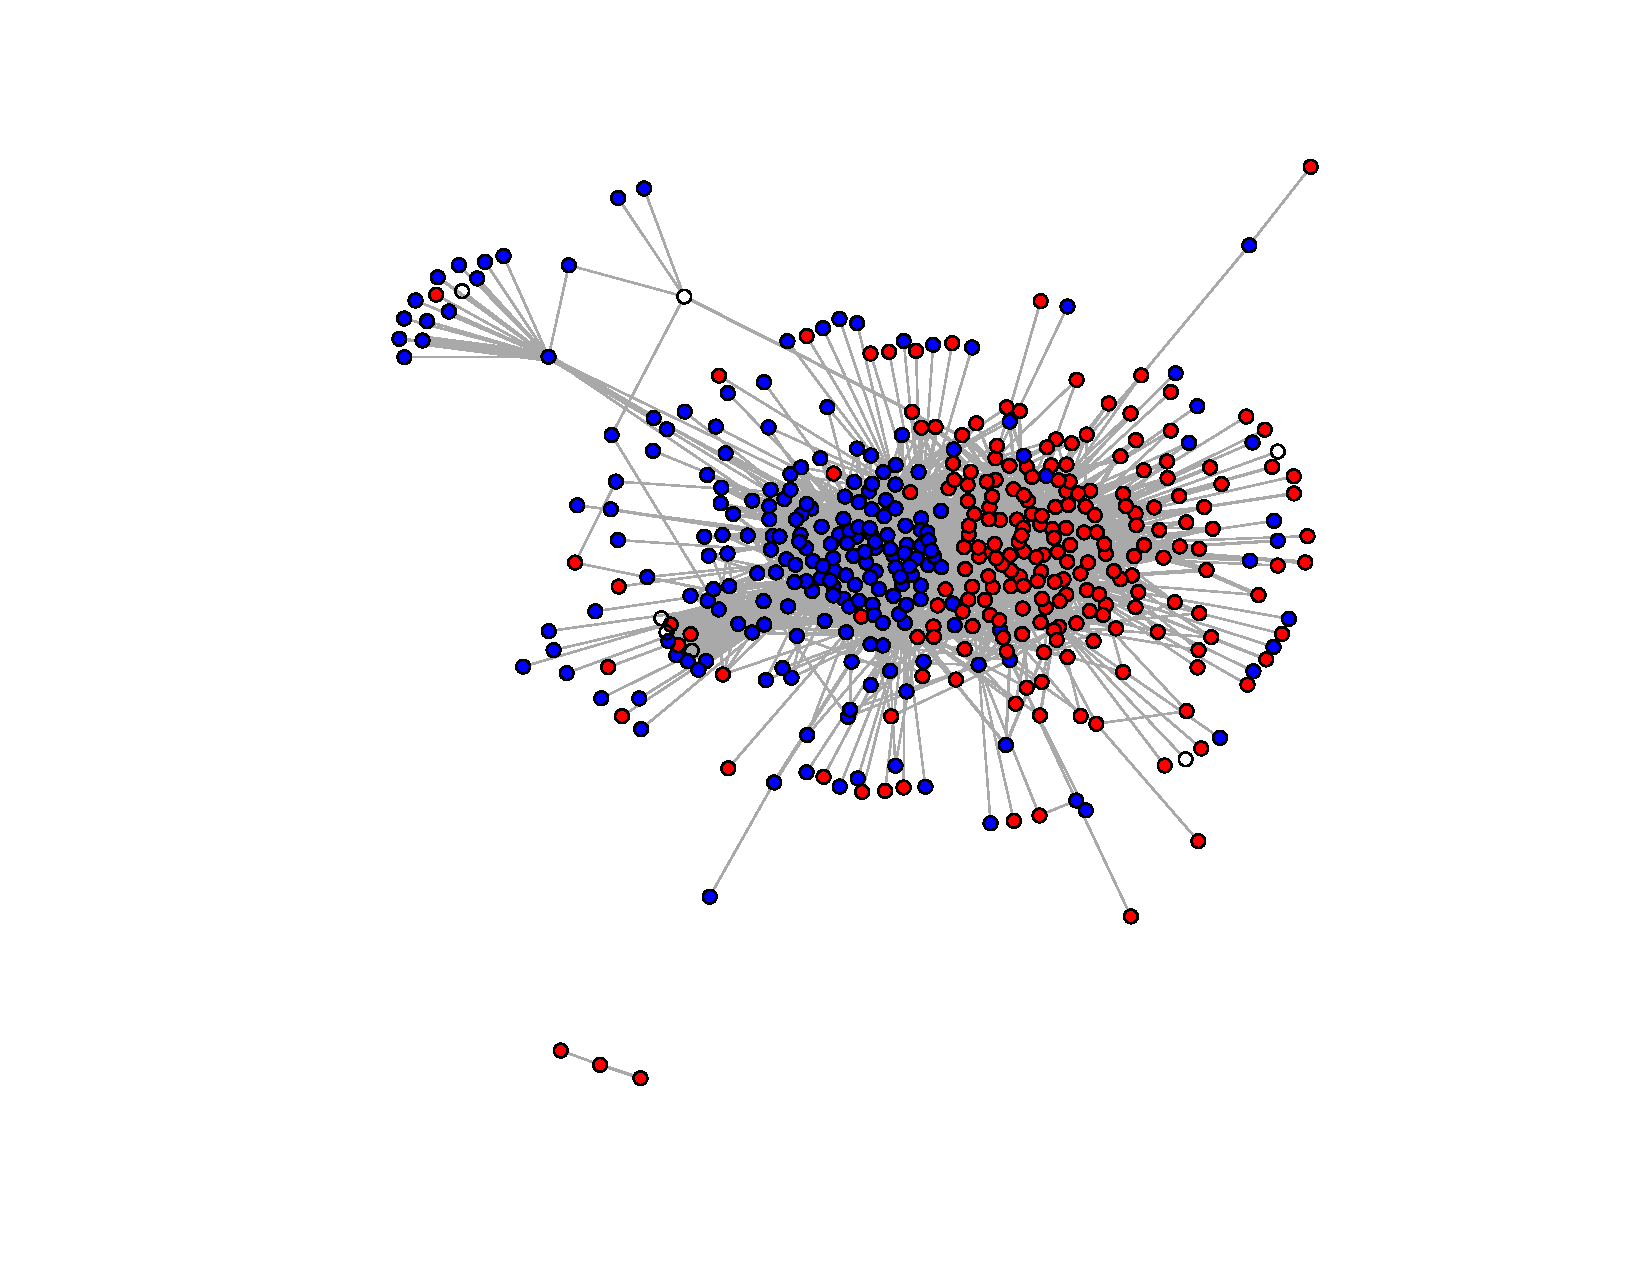
\includegraphics[width=.8\textwidth]{tweet_sharing_network.pdf}
\caption{Network of similar tweeters}
\label{fig:tweetnet}
\end{figure}

Of course much more work would be needed to test the association between tweet sharing and partisanship or other meaningful covariates like institutional position, geography, ideology, or issue interest rigorously. However this brief descriptive result serves to demonstrate the utility of SSW. This application of the technique produced a rich relational dataset that is well suited to testing further theories of congressional behavior. 

\section{Conclusion and Future Work}
This paper makes the case that coordination and cooperation is a central issue in the study of elite political actors generally and the study of congressional behavior in particular. In it I have presented a substantively meaningful extension of a text reuse detection tool that is better suited for detecting instances of reuse where the text has been adapted to suit new circumstances or new contexts. 

The method details a manner for weighting misalignments in text strings according to semantically meaningful differences. This paper has demonstrated the usefulness of this technique by inferring a message-sharing network in a corpus of tweets by Congress Members and candidates. There is notably partisan, and there is much more apparent message overlap between members than candidates.

While the version presented here is a comparatively simple implementation, the method is highly extensible and can ultimately enable much more sophisticated and context sensitive weighting. For example, in the type of semantic word embeddings used here,\texttt{word2vec}, \cite{mikolov2013linguistic} have observed semantically meaningful regularities in the vector space. That is, words pairs with the analogous semantic relationships (e.g. comparative::superlative) tend to have similar offsets as each other in vector the vectors space. It may be possible, then, to identify the offset relationship between compulsory and non-compulsory words, and weight the dimensions in which that offset occurs highly. This would allow for a version of SSW that could appropriately account for the small but extremely significant change of ``shall" to ``may" in a bill.


% Please add the following required packages to your document preamble:
% \usepackage[normalem]{ulem}
% \useunder{\uline}{\ul}{}
\begin{table}[]
\tiny
\centering
\caption{Tweet pairs with SW above 90 and SSW above 105}
\label{tbl:diff}
\begin{tabular}{|p{.03\columnwidth}|p{.04\columnwidth}|p{.42\columnwidth}|p{.42\columnwidth}|}
\hline
SW Score & SSW Score & Query Tweet                                                                                                                                              & Response Tweet                                                                                                                                            \\ \hline
100      & 129.17    & Thank you to all brave men and women serving our nation and keeping us safe. \#ArmedForcesDay https://t.co/xVswnTWMR0                                    & Thank you to all of the brave men and women who serve our country and keep us safe. \#ArmedForcesDay                                                      \\ \hline
110      & 134.63    & My thoughts and prayers are with the victims, their families and all those affected by the attack in Orlando.                                            & My thoughts and prayers are with the victims, the injured, their families and all others impacted by today's senseless attacks in \#Boston.               \\ \hline
95       & 118.66    & My staff and I are safe and praying for anyone who may be injured. Thankful for the U.S. Capitol Police and their swift actions today. \#GA08            & My staff and I are safe and accounted for. Praying for those who may have been hurt and grateful to the Capitol Police.                                   \\ \hline
105      & 126.79    & Today is \#equalpayday-50 years after the enactment of the Equal Pay Act, women still earn just 77 cents to every dollar a man earns.                    & 51 years after passage of the Equal Pay Act, a woman still earns 77 cents for every dollar a man earns. This is unacceptable \#NoMadMenPay                \\ \hline
110      & 131.26    & \#LWCF has preserved our natural \& cultural heritage for 50yrs. We must reauthorize this essential tool for conserving iconic \#publiclands         & \#LWCF has preserved our natural \& cultural heritage for 50 yrs. We should embrace this tool to conserve iconic \#publiclands                        \\ \hline
110      & 131.26    & \#LWCF has preserved our natural \& cultural heritage for 50yrs. We must reauthorize this essential tool for conserving iconic \#publiclands         & \#LWCF has preserved our natural \& cultural heritage for 50 yrs. We should embrace this tool to conserve iconic \#publiclands                        \\ \hline
110      & 131.26    & \#LWCF has preserved our natural \& cultural heritage for 50yrs. We must reauthorize this essential tool for conserving iconic \#publiclands         & \#LWCF has preserved our natural \& cultural heritage for 50 yrs. We should embrace this tool to conserve iconic \#publiclands                        \\ \hline
110      & 131.26    & \#LWCF has preserved our natural \& cultural heritage for 50yrs. We must reauthorize this essential tool for conserving iconic \#publiclands         & \#LWCF has preserved our natural \& cultural heritage for 50 yrs. We should embrace this tool to conserve iconic \#publiclands                        \\ \hline
100      & 121.15    & My thoughts and prayers are with the victims of this unspeakable tragedy in Boston and their families.                                                   & Thoughts and prayers are with the victims of the horrific attack in Orlando and their families.                                                           \\ \hline
95       & 115.97    & I am shocked to hear of the horrific explosions in Boston today. My thoughts are with the victims \& families \& the brave first responders.     & I am deeply saddened to hear about the tragedy in \#Orlando. My thoughts are with the victims, their families, and the city.                              \\ \hline
105      & 125.52    & \#ObamaBudget by the numbers: \$964 billion in new spending, \$1.1 trillion in new taxes \& \$8.2 trillion in new debt. Americans deserve better       & President Obama’s \#budget by the numbers: \$8.2 trillion in new debt, \$1.1 trillion in new taxes, \& \$964 billion in new spending.                   \\ \hline
105      & 125.52    & \#ObamaBudget by the numbers: \$964 billion in new spending, \$1.1 trillion in new taxes \& \$8.2 trillion in new debt. Americans deserve better       & President Obama’s \#budget by the numbers: \$8.2 trillion in new debt, \$1.1 trillion in new taxes, \& \$964 billion in new spending.                   \\ \hline
95       & 114.95    & Wishing all of the moms out there a very happy Mother's Day. Thank you for all you do! \#happymothersday https://t.co/DqhlqdtDq4                         & I want to wish all of the dads a very Happy Father’s Day and thank you for everything you do. https://t.co/In5sXa8bi6                                     \\ \hline
115      & 134.77    & My thoughts and prayers are with the families of the two officers who were slain in Des Moines, Iowa.                                                    & My thoughts and prayers are with the families of the five warriors who were killed in today's helicopter crash in... http://t.co/Zu0OiOAff3               \\ \hline
95       & 114.16    & \#Friedrichs decision is a victory for fair access to union representation, but we must stay vigilant against attacks on organized labor.                & SCOTUS \#Friedrichs tie decision is a win for union representation \& workers. We must remain strong against attacks on organized labor.              \\ \hline
95       & 113.48    & My thoughts and prayers are with everyone impacted by the tornadoes in Oklahoma.                                                                         & My thoughts and prayers are with all those impacted by the tornado in Oklahoma.                                                                           \\ \hline
110      & 128.06    & This morning my thoughts and prayers are with the people of Oklahoma and all those affected by yesterday's tornado. \#PrayforOklahoma                    & RT@SpeakerBoehner: Our thoughts and prayers are with the people of Japan and all those impacted by this morning’s disaster.                               \\ \hline
110      & 127.88    & Today is the last day to register to vote in the November 3rd elections in Virginia. Here's more information: https://t.co/DZ5I9uQbuJ                    & Today is the last day to register to vote in the Nov election in GA. Don't be left out or left behind, register today http://t.co/1G4uOQdd20              \\ \hline
120      & 137.76    & \#Energy \& \#Manufacturing go hand in hand. Lower energy costs keep \#USA manufacturers competitive, and create \#jobs. | \#NationOfBuilders        & \#Energy \& \#manufacturing go hand in hand. Lower energy costs keeps U.S. manufacturers competitive \& creates \#jobs \#NationOfBuilders         \\ \hline
120      & 137.76    & \#Energy \& \#Manufacturing go hand in hand. Lower energy costs keep \#USA manufacturers competitive, and create \#jobs. | \#NationOfBuilders        & \#Energy \& \#manufacturing go hand in hand. Lower energy costs keeps U.S. manufacturers competitive \& creates \#jobs \#NationOfBuilders         \\ \hline
100      & 117.36    & \#Startups are creating \#jobs \& supporting \#innovation. RT to give them the recognition they deserve! \#StartupDay http://t.co/P9cdZlkEkL         & \#Startups create \#jobs here in \#MA03 \& support \#innovation. RT to give them recognition they deserve! \#StartupDay http://t.co/7TF0fIyi5a        \\ \hline
95       & 112.36    & Start-up companies are creating jobs \& supporting innovation. RT to give them recognition they deserve! \#StartupDay http://t.co/ttZ7TtAhqi         & Happy \#StartupDay! Startup companies create \#jobs \& support \#innovation. RT to give them recognition they deserve! https://t.co/8fKmjO0RPv        \\ \hline
115      & 132.24    & I believe Congress should do the job it was elected to do, or they should not be paid. \#NE02 https://t.co/vty3zwlpho                                    & Members of Congress must do the job they were elected to do, or they should not be paid. RT if you agree. https://t.co/8Wtsq9MYwg                         \\ \hline
\end{tabular}
\end{table}







\begin{table}[]
\tiny
\centering
\caption{More Tweet pairs with SW above 90 and SSW above 105}
\label{tbl:diff2}
\begin{tabular}{|p{.03\columnwidth}|p{.04\columnwidth}|p{.42\columnwidth}|p{.42\columnwidth}|}
\hline
SW Score & SSW Score & Query Tweet                                                                                                                                              & Response Tweet                                                                                                                                            \\ \hline
105      & 122.23    & Sad to hear of the terror attack against innocent civilians in \#TelAviv \#Israel. My thoughts \& prayers are with the victims \& their families & I condemn the vicious terrorist attack against innocent worshipers in \#Jerusalem. My thoughts \& prayers are with the victims' families.             \\ \hline
95       & 112.17    & We can invest in young girls by addressing reproductive health, education, livelihoods, \& civic engagement. \#YouthDay \#SRHR                       & We must invest in girls w/ approaches that address sexual \& reproductive health, education, livelihoods, \& civic engagement! \#YouthDay \#SRHR  \\ \hline
100      & 117.14    & I stand with \#LGBT Ukrainians celebrating \#OdessaPride2016. No one should be targeted because of who they are or who they love.                        & As we mark LGBT Pride Month, we are reminded that no one should ever be a target because of who they are or whom they love.                               \\ \hline
110      & 126.97    & Today is the 79th anniversary of \#SocialSecurity, a crucial part of \#SocialSafetyNet for many deserving Americans that we must protect!                & Today is 79th anniv of \#SocialSecurity, a critical part of the \#SocialSafetyNet for millions of hard-working Americans that we must protect!            \\ \hline
130      & 146.97    & Today is the 79th anniversary of \#SocialSecurity, a crucial part of \#SocialSafetyNet for many deserving Americans that we must protect!                & Today is the 79th anniv of \#SocialSecurity, a critical part of \#SocialSafetyNet for millions of hard-working Americans that we must protect!            \\ \hline
100      & 116.51    & It's past time to \#DisarmHate. Tomorrow as LGBTQ \& gun violence prevention groups unite to demand action, I stand with them \#DisarmHateRally      & Tomorrow LGBTQ \& gun violence prevention advocates are uniting in DC to demand action. I stand with them \#DisarmHate https://t.co/M1bibV69SV        \\ \hline
100      & 116.51    & It's past time to \#DisarmHate. Tomorrow as LGBTQ \& gun violence prevention groups unite to demand action, I stand with them \#DisarmHateRally      & Tomorrow LGBTQ \& gun violence prevention advocates are uniting in DC to demand action. I stand with them \#DisarmHate https://t.co/adHJL27B0Z        \\ \hline
100      & 116.51    & It's past time to \#DisarmHate. Tomorrow as LGBTQ \& gun violence prevention groups unite to demand action, I stand with them \#DisarmHateRally      & Tomorrow LGBTQ \& gun violence prevention advocates are uniting in DC to demand action. I stand with them \#DisarmHate https://t.co/VGO27MOimg        \\ \hline
105      & 121.40    & On Pearl Harbor Remembrance Day, we honor those who have served and sacrificed for our country. http://t.co/1uzTNA2j6K                                   & As the son of a WWII vet, on Pearl Harbor Remembrance Day we honor all who served \& sacrificed for our great nation. http://t.co/f9kscuCdW1          \\ \hline
120      & 136.19    & Of course, we still have a lot more work to do to make sure that veterans get the care they deserve, and I'll continue to stay on it.                    & The VA still has a lot of work to do to make sure that our Veterans are getting the care they've earned and deserve! https://t.co/Rj3o9iU2jh              \\ \hline
95       & 110.94    & Did you know the govt paid \$1.2 million to pay people to play World of Warcraft? http://t.co/Nrg000gx Instead of tax hikes \#CutWaste                   & Tax dollars at work: govt paid \$1.2 mil to study seniors playing World of Warcraft http://t.co/YVJvGUA1 Instead of tax hikes \#CutWaste                  \\ \hline
125      & 140.81    & For 40 years the Hyde Amendment has told women that USA laws \& rights don't apply equally to us. We must \#BeBoldEndHyde                            & For 4 decades, the Hyde Amendment has told women that our laws + rights don't apply equally to them. It is time to \#BeBoldEndHyde.                       \\ \hline
95       & 110.60    & Our thoughts and prayers go out to the families and victims of the devastating shooting yesterday in Kansas City,... http://t.co/mSarFd3zJ4              & My thoughts and prayers go out to the family and friends of the victims of the tragic school shooting in Connecticut this morning.                        \\ \hline
105      & 120.50    & More than 88,000 people in Illinois lost unemployment insurance. It’s unacceptable that House GOP refuse to allow a vote to \#RenewUI.                   & Since Dec. 62,915 people in \#Massachusetts have lost unemployment insurance because House GOP refuses to allow a vote to \#RenewUI.                      \\ \hline
110      & 125.47    & Our thoughts \& prayers are with the friends \& family of Officer Jacai Colson in the midst of this tragedy. https://t.co/fTpPx92ON7             & My thoughts \& prayers are with the family \& friends of Officer Jacai Colson, who was killed in the line of duty today, \& @PGPDNews family. \\ \hline
105      & 120.40    & My deepest condolences go out to the families and friends of the victims of this morning’s tragic shooting at the \#DCNavyYard.                          & My thoughts and prayers go out to the family and friends of the victims of the tragic school shooting in Connecticut this morning.                        \\ \hline
105      & 120.34    & You have 9 days left to get your submissions in for this year’s Congressional Art Competition. Details here --\&gt; http://t.co/nHS1IEkHZq               & \#NY21 High School Students: You have just 3 days left to get your entries in for the Congressional Art Competition https://t.co/Fa6lNmF1Xs               \\ \hline
170      & 185.26    & A veto on the \#FY16NDAA withholds support and resources our troops and our nation needs. Mr. President, it's up to you to \#SignTheBill.                & A veto on this bill withholds support and resources that our troops and our nation need. Mr. President, it's up to you to \#SignTheBill                   \\ \hline
95       & 110.19    & May is Military Appreciation Month. Thank you to our men and women in uniform who defend freedom each day. VIDEO: http://t.co/xlEfFYhuzm                 & Thank you to all of our men and women in uniform who protect our freedom every day \#ArmedForcesDay https://t.co/aBEK4xXho7                               \\ \hline
95       & 110.16    & Happy Mothers Day to my mom Carmen and all mothers. Thank you for everything you do! https://t.co/HiHmUvZYdy                                             & Wishing a Happy Mother's Day to my Mom and all of the amazing Moms today. Thank you for everything you do for us! https://t.co/LlEuEafpKM                 \\ \hline
115      & 130.04    & My thoughts and prayers are with the victims and loved ones of this morning's tragic shooting in Orlando                                                 & My thoughts and prayers are with the victims and their loved ones of the horrific attack in Orlando.                                                      \\ \hline
110      & 124.89    & My thoughts and prayers are with the people of Japan and those affected by the earthquake and tsunami. If you have... http://fb.me/TlBlz6hF              & RT@SpeakerBoehner: Our thoughts and prayers are with the people of Japan and all those impacted by this morning’s disaster.                               \\ \hline
110      & 124.89    & My thoughts and prayers are with the people of Japan and those affected by the earthquake and tsunami. If you have... http://fb.me/TlBlz6hF              & RT@SpeakerBoehner: Our thoughts and prayers are with the people of Japan and all those impacted by this morning’s disaster.                               \\ \hline
105      & 119.72    & The @HouseGOP decided to let @ExImBankUS shut down even though it puts American jobs at risk. RT to show your support for \#ExIm4Jobs                    & .@HouseGOP decided to \#EndExIm even though shutting down @ExImBankUS will put American jobs at risk. RT to show your support for \#ExIm4Jobs.            \\ \hline
105      & 119.72    & The @HouseGOP decided to let @ExImBankUS shut down even though it puts American jobs at risk. RT to show your support for \#ExIm4Jobs                    & .@HouseGOP decided to \#EndExIm even though shutting down @ExImBankUS will put American jobs at risk. RT to show your support for \#ExIm4Jobs.            \\ \hline
150      & 164.68    & From literacy tests to cutting early voting. From poll taxes to unnecessary voter IDs. Our county has more to do. \#RestoreTheVRA \#VRA50                & From literacy tests to cutting early voting, poll taxes to unnecessary voter IDs We have more to do. \#RestoreTheVRA http://t.co/KLt7RJjZ6F               \\ \hline
\end{tabular}
\end{table}
%TCIMACRO{%
%\TeXButton{endnotes}{\newpage
%\begingroup
%\renewcommand{\enotesize}{\normalsize}
%\theendnotes
%\endgroup}}%
%BeginExpansion
\newpage
\begingroup
\renewcommand{\enotesize}{\normalsize}
\theendnotes
\endgroup%
\pagebreak

\bibliographystyle{kluwer}
\bibliography{sigproc}



%TCIMACRO{\TeXButton{endflushleft}{\end{flushleft}}}%
%BeginExpansion
\end{flushleft}%
%EndExpansion
\pagebreak

\end{document}